% -*- mode: latex; mode: auto-fill -*-
\documentclass[a4paper,12pt,oneside]{book}
\usepackage[doublespacing]{setspace}
\usepackage[a4paper, margin=1.5in, top=1in, bottom=1in,
  bindingoffset=0cm, includehead=true, includefoot=true]{geometry}
\usepackage{microtype}
\usepackage{emptypage}
\usepackage{ragged2e} % for \RaggedRight
\usepackage{hyperref}
%\usepackage[hyphenbreaks]{breakurl}
\usepackage{fancyhdr}
\usepackage{color}
\usepackage{enumitem}
\usepackage{graphicx}
\usepackage{float}
\usepackage{listings}

\usepackage{etoolbox}
\AtBeginEnvironment{minted}{\singlespacing%
  \fontsize{8}{8}\selectfont}
\AtBeginEnvironment{enumerate}{\singlespacing}
\AtBeginEnvironment{figure}{\singlespacing}

\definecolor{MyBlue}{RGB}{6, 69, 173}
\hypersetup{
  colorlinks,
  linkcolor=MyBlue,
  urlcolor=MyBlue,
  citecolor=MyBlue
}

\fancyhf{}
\fancyhead[LE]{\nouppercase{\leftmark}}
\fancyhead[RO]{\nouppercase{\rightmark}}
\fancyfoot[C]{\thepage}

%\usepackage{breakurl}

\begin{document}
\frontmatter
\pagestyle{empty}

\phantomsection
\addcontentsline{toc}{chapter}{Cover}
\clearpage
\begin{center}
  \bfseries
  \large
  \vspace*{\stretch{1}}

  {\LARGE Your FYP Title}\\
  BY\\
  {\Large Your Name}\\

  \vspace*{\stretch{3}}

  Final Year project submitted in partial fulfilment of the
  requirements for the Degree of\\
  Bachelor of Science in Computer Science

  \vspace*{\stretch{3}}

  Department of Computer Science\\
  School of Sciences and Engineering\\
  University of Nicosia\\
  June 2026
\end{center}
\pagebreak

\phantomsection
\addcontentsline{toc}{chapter}{Signatures}
\clearpage
\normalsize
\begin{center}
{\bf
{\large Your FYP Title}\\
{\normalsize BY}\\
{\large Your Name}\\}
\smallbreak
This Final Year Project has been accepted in partial fulfilment of the
requirements for the Degree of\\
Bachelor of Science in Computer Science
\end{center}
\vspace*{\stretch{1}}

\noindent Project Advisor:\\
\mbox{\par\noindent\makebox[3.0in]{\hrulefill} \hspace*{0.1in}
\hfill\makebox[1.5in]{\hrulefill} \hspace*{0.1in}
\hfill\makebox[0.3in]{\hrulefill}/\hfill\makebox[0.3in]{\hrulefill}/\hfill\makebox[0.3in]{\hrulefill}}\\
\mbox{\par\noindent\makebox[3.0in]{(Name)} \hspace*{0.1in}
\hfill\makebox[1.5in]{(Signature)} \hspace*{0.1in}
\hfill\makebox[1.1in]{(Date)}}\\
\\
\noindent Examiner:\\
\mbox{\par\noindent\makebox[3.0in]{\hrulefill} \hspace*{0.1in}
\hfill\makebox[1.5in]{\hrulefill} \hspace*{0.1in}
\hfill\makebox[0.3in]{\hrulefill}/\hfill\makebox[0.3in]{\hrulefill}/\hfill\makebox[0.3in]{\hrulefill}}\\
\mbox{\par\noindent\makebox[3.0in]{(Name)} \hspace*{0.1in}
\hfill\makebox[1.5in]{(Signature)} \hspace*{0.1in}
\hfill\makebox[1.1in]{(Date)}}\\
\\
\noindent Examiner:\\
\mbox{\par\noindent\makebox[3.0in]{\hrulefill} \hspace*{0.1in}
\hfill\makebox[1.5in]{\hrulefill} \hspace*{0.1in}
\hfill\makebox[0.3in]{\hrulefill}/\hfill\makebox[0.3in]{\hrulefill}/\hfill\makebox[0.3in]{\hrulefill}}\\
\mbox{\par\noindent\makebox[3.0in]{(Name)} \hspace*{0.1in}
\hfill\makebox[1.5in]{(Signature)} \hspace*{0.1in}
\hfill\makebox[1.1in]{(Date)}}

\vspace*{\stretch{2}}
\begin{center}
\bfseries
Department of Computer Science\\
School of Sciences and Engineering\\
University of Nicosia
\end{center}
\pagebreak

\cleardoublepage
\phantomsection
\addcontentsline{toc}{chapter}{Abstract}
\raggedbottom
\par\noindent{\bf\Huge Abstract}\\

\noindent The purpose of this project is to 
\pagebreak

\phantomsection
\addcontentsline{toc}{chapter}{Acknowledgements}
\raggedbottom
\par\noindent{\bf\Huge Acknowledgements}\\

\noindent I would like to thank ...


\raggedbottom % don't stretch vertically
\cleardoublepage
\phantomsection
\addcontentsline{toc}{chapter}{Table of Contents}
\pagestyle{plain}
\newgeometry{includehead=false,includefoot=false}
\begingroup
\singlespacing
\tableofcontents

\newpage
\listoffigures
\newpage
\listoftables

\endgroup
\restoregeometry

\mainmatter
\pagestyle{fancy}

%%%%%%%%%%%%%%%%%%%% Chapter ONE %%%%%%%%%%
\chapter{Introduction}
In our era ...


\section{What is a kernel}
The kernel is

%% Roadmap of the rest of the thesis
The rest of the thesis is organized as follows: Chapter \ref{sec:overview}, describes how to build the development environment. Chapter \ref{} , describes how.... Finally, Chapter \ref{sec:con} concludes the report.

%%%%%%%%%%%%%%%%%%%% Chapter TWO %%%%%%%%%%
\chapter{Overview of ...}
\label{sec:overview}
In this chapter the hard

\section{Hardware requirements}
The following are the hardware requirements \cite{ewmaintrusiondetection} ..:

\section{Software dependencies}
This section describes..

Figure \ref{fig:lvl_2_entries} illustrates ...

\begin{enumerate}
\item Fault, that means the entry does not point anywhere   (i.e. invalid memory address).
\item Large page, that points to a physical address of 64KB memory region.
\item Small page, that points to a physical address of 4096B (4KB)   memory region.
\end{enumerate}

\begin{figure}[H]
  \centering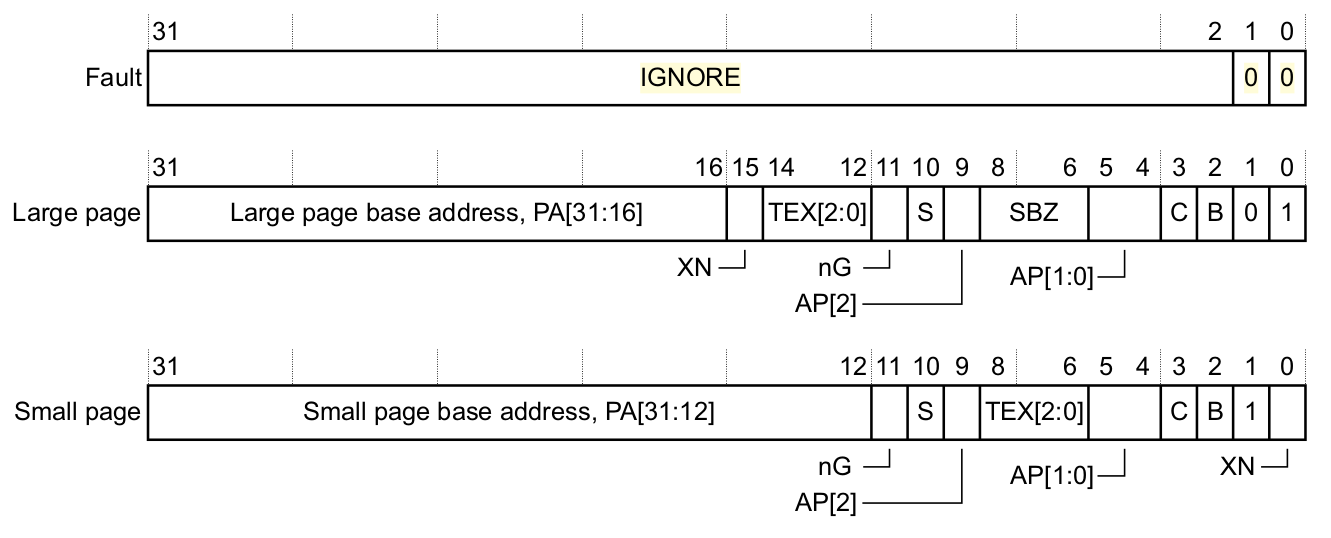
\includegraphics[scale=0.3]{images/mmu_2nd_level.png}
  \caption{Second-Level Entries}
  \label{fig:lvl_2_entries}
\end{figure}

For simplicity the kernel is using only the {\bf Small page} descriptor and {\bf Fault} descriptor for invalid adresses. 

The following code invalidates the TLB.

\begin{lstlisting}
asm volatile (
        /* invalidate TLB
         * v1 is ignored by the CP15 */
        "mcr p15, 0, v1, c8, c7, 0      \n\t"
        /* completes the TLB invalidation */
        "dsb                            \n\t"
        : : : "v1", "memory"
);
\end{lstlisting}


%%%%%%%%%%%%%%%%%%%% Chapter THREE %%%%%%%%%%
\chapter{Processes}
\label{sec:processes}
This chapter describes how the kernel creates new threads, how they are scheduled and how the can sleep/wakeup.

\section{Threads}
Kernel implements only kernel-level threads, every thread has its own {\it task\_struct} struct which has the following fields:

\begin{lstlisting}
struct task_struct {
        pid_t pid;
        task_state_t state;
        sleep_reason_t sleep_reason;
        u32 sleep_chan;
        volatile int scheduled;
        struct regs regs;
        struct list_head list;
        void *stack_alloc;
        u32 wakeup_ms;
};
\end{lstlisting}

\begin{enumerate}
  \item {\bf pid} is the process id, every thread have different
    process id.
  \item {\bf state} is the current state of the thread, it can can get the
    following values:
    \begin{enumerate}[label*=\arabic*]
      \item {\bf TASK\_TERMINATE} is when the thread had exited and
        must be removed from the list.
      \item {\bf TASK\_RUNNABLE} is when the thread can run.
      \item {\bf TASK\_RUNNING} is when the thread is running.
      \item {\bf TASK\_SPLEEPING} is when the thread is sleeping for a
        reason.
    \end{enumerate}
    \item {\bf sleep\_reason} is the reason that the the thread is
      sleeping, it can get the following values:
      \begin{enumerate}[label*=\arabic*]
        \item {\bf SLEEPR\_SLEEP} is when the thread called the {\it
          sleep} function.
        \item {\bf SLEEPR\_SUSPEND} is then the thread suspend
          (i.e. sleep) itself until some other thread resume it
          (i.e. awakes it), for example when semaphore is released.
      \end{enumerate}
    \item {\bf sleep\_chan} is the id that the other thread must use
      to resume the thread.
    \item {\bf scheduled} is true if the thread has ben scheduled.
    \item {\bf regs} are all the registers that context switch saves.
    \item {\bf list} has the next and the previous {\bf task\_struct}.
    \item {\bf stack\_alloc} has the memory region of thread's stack.
    \item {\bf wakeup\_ms} has what time must a thread wakeup from sleep.
\end{enumerate}


%%%%%%%%%%%% END%%%%%%%%%%%%%%
\chapter{Conclusion and future work}
\label{sec:con}

This thesis has presented an \cite{springer2020} implementation

%% bibliography
\bibliographystyle{unsrt}
% \nocite{*}
% \begingroup
% \RaggedRight % Avoid justification in bibliography leading to too much space.
\bibliography{thesis}
% \endgroup



\end{document}
